\section{Limitations}
First, as we add more robots or obstacles to our model, the algorithm would become increasingly lengthy. For each new robot added, we need to add one term for each existing differential equation and two new differential equations. For each new obstacle added, we need to add one term for each existing differential equation. The result is a boilerplate. Therefore, in the future, we could improve the algorithm by methods like reusing variables, employing automatic code generation, etc.

Second, we did not treat the obstacles in our model as an object that is repulsive in every differential part -- rather, it is a hollow ring. That means sometimes, crossing the ring may actually be less costly for the robots (in part due to the deficiency of numerical methods). Hence, if the repulsiveness of the obstacles are not weighted up, the following situation could occur (for case 10.4); however, it can be amended by adjusting weight of repulsiveness of obstacles. 
\begin{figure}[H]
    \centering
    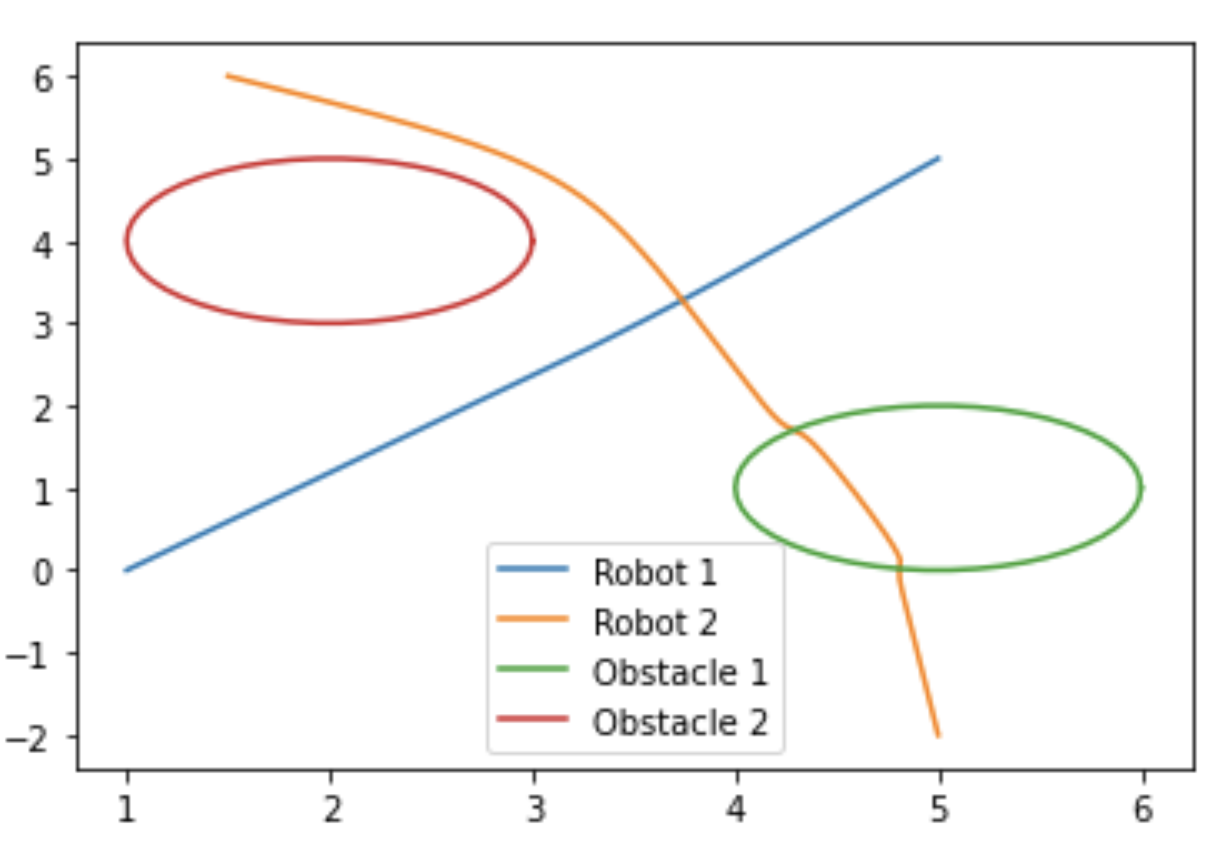
\includegraphics[width=10cm]{Graphs/limitation.png}
    \label{fig:my_label}
\end{figure}
\section{Summary}

To conclude, our model appears to be robust and provides a reasonable approximation of the robots' optimal trajectories. Indeed, the trial cases result in the expected trajectories: in case 1, straight lines are produced, and in all the other cases, the robots never hit each other or the obstacle. Notably, splitting the cost functional into three sub-parts proved advantageous as it allows the weight of the conditions to be manipulated if needed. For example, if desired, one could easily further increase the distance away from the obstacles that the robots are by increasing the weight of the repulsiveness of the obstacles. Indeed, by removing the square root in our length function for the purposes of computation, we increased the prioritization of a shorter path versus not crashing into the obstacles. To offset this, we weighted the repulsiveness higher as well. Overall, the perhaps counter intuitive approach of treating the robots and obstacles as charges seams to be sound. 

Given the opportunity for future research, we would seek out a way to program the unsimplified version of our length function (keeping the square root rather than omitting it) in order to produce more reliably accurate results without having to manipulate the weight of each part of the functional. This would require coding our own differential equation solver in Python since the current functions available do not support that type of equation. Another avenue of future exploration could be modifying the problem to have different constraints. For example, rather than just having the robots not crash into each other, we could say that they must maintain a specific minimum distance apart from each other. This would add another condition on the position of the robots beyond just the start and stop boundary conditions. Alternatively, we could also focus on changing the problem to better reflect real life applications. For example, we could extend the model to accommodate 3 dimensions rather than the 2D plane and give the robots a non-negligible volume rather than treating them as point particles. This would necessitate formulating the question as an optimal control problem. 



\section{Contributions}
\begin{itemize}
    \item \textbf{Lance Remigio:} Case analysis, plotting, author of LaTex Document.
    \item \textbf{Jin Zhang:} Write algorithm, solving the differential equations numerically.
    \item \textbf{Fatma Djellouli:} Model formulation and first-order necessary conditions derivation.
    \item \textbf{Woody Lee:} Running test cases and construct limitations of the model. 
\end{itemize}
